% TikZ scaffold; thumbnails in Figures/framework_frames/ are LOW-RES CROPS of the
% old framework.png -- regenerate from the original matplotlib outputs (same
% filenames) for print quality. Prompt-template text moved to Appendix~B.
\resizebox{\textwidth}{!}{%
\begin{tikzpicture}[font=\small, >=Latex,
  photo/.style={inner sep=1pt, draw=gray!40, thin},
  blk/.style={rounded corners, draw, thick, align=center, inner sep=3pt,
              minimum height=8mm, font=\small},
  lbl/.style={font=\scriptsize, align=center},
  panel/.style={font=\small\bfseries, anchor=west},
]
% =============== (a) feature engineering (top) ===============
\node[blk, text width=24mm] (prompt)
  {task prompt\\ \scriptsize(Appendix~\ref{app:feature})};
\node[blk, right=8mm of prompt] (llm) {LLM};
\node[blk, right=8mm of llm, text width=22mm] (fsel) {candidate\\ features $F_{\text{sel}}$};
\node[blk, right=8mm of fsel, text width=30mm] (mi)
  {sufficiency check\\ $I(X_{\text{sel}};Y)\ge(1-\epsilon)I(X_{\text{raw}};Y)$};
\node[blk, right=8mm of mi, text width=26mm] (minz)
  {MI minimization:\\ drop redundant\\ features};
\node[blk, right=8mm of minz, fill=teachbg, text width=20mm] (fmin)
  {$F_{\min}$, $\mathcal{X}_{\min}$\\ \scriptsize fixed for all rounds};
\draw[->, thick] (prompt) -- (llm);
\draw[->, thick] (llm) -- (fsel);
\draw[->, thick] (fsel) -- (mi);
\draw[->, thick] (mi) -- node[above, font=\scriptsize]{pass} (minz);
\draw[->, thick] (minz) -- (fmin);
\draw[->, thick, dashed] (mi.south) -- ++(0,-4.5mm) -| node[below, pos=0.25, font=\scriptsize]
  {fail: user refines task description} (prompt.south);
\node[panel] at ([xshift=-2mm,yshift=4mm]prompt.north west)
  {(a) Two-stage feature engineering = observability certificate for Assumption~\ref{as:obs} (Sec.~\ref{sec:feature_engineering})};
% =============== (b) active learning loop (bottom) ===============
\node[photo, below=17mm of prompt.south west, anchor=north west] (demos) {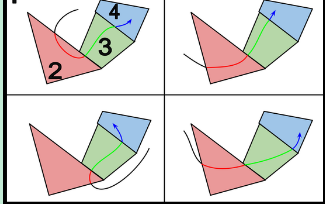
\includegraphics[height=2.1cm]{Figures/framework_frames/demos.png}};
\node[photo, right=13mm of demos] (weak) {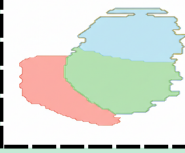
\includegraphics[height=2.1cm]{Figures/framework_frames/weak.png}};
\node[photo, right=13mm of weak] (uncert) {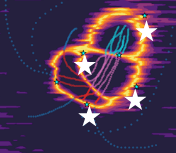
\includegraphics[height=2.1cm]{Figures/framework_frames/uncert.png}};
\node[photo, right=13mm of uncert] (queried) {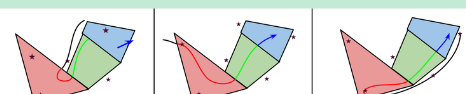
\includegraphics[height=1.35cm]{Figures/framework_frames/queried.png}};
\node[photo, right=13mm of queried] (strong) {
\includegraphics[height=2.1cm]{Figures/framework_frames/strong.png}};
\node[lbl, below=1mm of demos]  {initial segmented\\ demos $\mathcal{D}_0$};
\node[lbl, below=1mm of weak]   {weak classifier};
\node[lbl, below=1mm of uncert] {acquisition $\alpha$,\\ query points $X_K$};
\node[lbl, below=1mm of queried]{safe demos through $X_K$};
\node[lbl, below=1mm of strong] {strong classifier $f$};
\draw[->, thick] (demos) -- node[above, font=\scriptsize]{train} (weak);
\draw[->, thick] (weak) -- (uncert);
\draw[->, thick] (uncert) -- node[above, font=\scriptsize]{\faUser} (queried);
\draw[->, thick] (queried) -- node[above, font=\scriptsize]{retrain} (strong);
\node[panel] at ([xshift=-2mm,yshift=5mm]demos.north west)
  {(b) Active learning of the localizer (Algorithm~\ref{alg:active})};
\end{tikzpicture}%
}
